\documentclass{extbook}[14pt]
\usepackage{multicol, enumerate, enumitem, hyperref, color, soul, setspace, parskip, fancyhdr, amssymb, amsthm, amsmath, bbm, latexsym, units, mathtools}
\everymath{\displaystyle}
\usepackage[headsep=0.5cm,headheight=0cm, left=1 in,right= 1 in,top= 1 in,bottom= 1 in]{geometry}
\usepackage{dashrule}  % Package to use the command below to create lines between items
\newcommand{\litem}[1]{\item #1

\rule{\textwidth}{0.4pt}}
\pagestyle{fancy}
\lhead{}
\chead{Answer Key for Progress Quiz 10 Version B}
\rhead{}
\lfoot{6232-9639}
\cfoot{}
\rfoot{Fall 2020}
\begin{document}
\textbf{This key should allow you to understand why you choose the option you did (beyond just getting a question right or wrong). \href{https://xronos.clas.ufl.edu/mac1105spring2020/courseDescriptionAndMisc/Exams/LearningFromResults}{More instructions on how to use this key can be found here}.}

\textbf{If you have a suggestion to make the keys better, \href{https://forms.gle/CZkbZmPbC9XALEE88}{please fill out the short survey here}.}

\textit{Note: This key is auto-generated and may contain issues and/or errors. The keys are reviewed after each exam to ensure grading is done accurately. If there are issues (like duplicate options), they are noted in the offline gradebook. The keys are a work-in-progress to give students as many resources to improve as possible.}

\rule{\textwidth}{0.4pt}

\begin{enumerate}\litem{
Determine the domain of the function below.
\[ f(x) = \frac{4}{25x^{2} -36} \]

The solution is \( \text{All Real numbers except } x = -1.200 \text{ and } x = 1.200. \), which is option C.\begin{enumerate}[label=\Alph*.]
\item \( \text{All Real numbers.} \)

This corresponds to thinking the denominator has complex roots or that rational functions have a domain of all Real numbers.
\item \( \text{All Real numbers except } x = a \text{ and } x = b, \text{ where } a \in [-30, -29] \text{ and } b \in [28, 31] \)

All Real numbers except $x = -30.000$ and $x = 30.000$, which corresponds to not factoring the denominator correctly.
\item \( \text{All Real numbers except } x = a \text{ and } x = b, \text{ where } a \in [-2.2, -0.2] \text{ and } b \in [0.2, 3.2] \)

All Real numbers except $x = -1.200$ and $x = 1.200$, which is the correct option.
\item \( \text{All Real numbers except } x = a, \text{ where } a \in [-2.2, -0.2] \)

All Real numbers except $x = -1.200$, which corresponds to removing only 1 value from the denominator.
\item \( \text{All Real numbers except } x = a, \text{ where } a \in [-30, -29] \)

All Real numbers except $x = -30.000$, which corresponds to removing a distractor value from the denominator.
\end{enumerate}

\textbf{General Comment:} Recall that dividing by zero is not a real number. Therefore the domain is all real numbers \textbf{except} those that make the denominator 0.
}
\litem{
Choose the equation of the function graphed below.

\begin{center}
    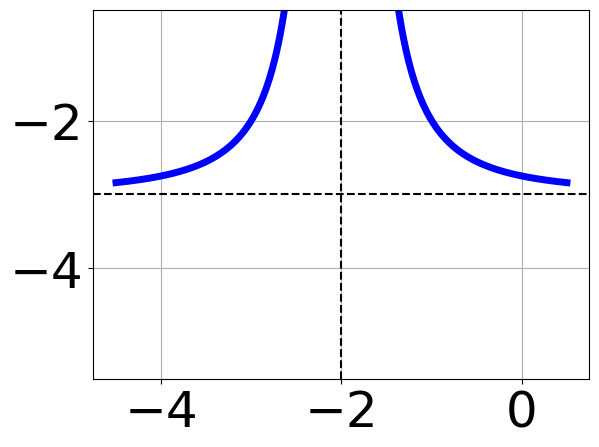
\includegraphics[width=0.5\textwidth]{../Figures/rationalGraphToEquationB.png}
\end{center}




The solution is \( \text{None of the above as it should be } f(x) = \frac{1}{(x + 2)^2} - 3 \), which is option E.\begin{enumerate}[label=\Alph*.]
\item \( f(x) = \frac{-1}{x + 2} - 3 \)

Corresponds to thinking the graph was a shifted version of $\frac{1}{x}$, using the general form $f(x) = \frac{a}{(x-h)^2}+k$, and the opposite leading coefficient.
\item \( f(x) = \frac{-1}{(x + 2)^2} - 3 \)

Corresponds to using the general form $f(x) = \frac{a}{(x-h)^2}+k$ and the opposite leading coefficient.
\item \( f(x) = \frac{1}{x - 2} - 3 \)

Corresponds to thinking the graph was a shifted version of $\frac{1}{x}$.
\item \( f(x) = \frac{1}{(x - 2)^2} - 3 \)

The $x$-value of the equation does not match the graph.
\item \( \text{None of the above} \)

None of the equation options were the correct equation.
\end{enumerate}

\textbf{General Comment:} Remember that the general form of a basic rational equation is $ f(x) = \frac{a}{(x-h)^n} + k$, where $a$ is the leading coefficient (and in this case, we assume is either $1$ or $-1$), $n$ is the degree (in this case, either $1$ or $2$), and $(h, k)$ is the intersection of the asymptotes.
}
\litem{
Solve the rational equation below. Then, choose the interval(s) that the solution(s) belongs to.
\[ \frac{-4x}{-6x + 5} + \frac{-6x^{2}}{-30x^{2} +x + 20} = \frac{-2}{5x + 4} \]

The solution is \( \text{There are two solutions: } x = 0.283 \text{ and } x = -1.360 \), which is option D.\begin{enumerate}[label=\Alph*.]
\item \( \text{All solutions lead to invalid or complex values in the equation.} \)


\item \( x \in [-1.41,-1.22] \)


\item \( x_1 \in [0.19, 0.87] \text{ and } x_2 \in [-0.9,1.7] \)


\item \( x_1 \in [0.19, 0.87] \text{ and } x_2 \in [-4.7,-0.5] \)

* $x = 0.283 \text{ and } x = -1.360$, which is the correct option.
\item \( x \in [-0.9,-0.56] \)


\end{enumerate}

\textbf{General Comment:} Distractors are different based on the number of solutions. Remember that after solving, we need to make sure our solution does not make the original equation divide by zero!
}
\litem{
Solve the rational equation below. Then, choose the interval(s) that the solution(s) belongs to.
\[ \frac{40}{20x -35} + 1 = \frac{40}{20x -35} \]

The solution is \( \text{all solutions are invalid or lead to complex values in the equation.} \), which is option C.\begin{enumerate}[label=\Alph*.]
\item \( x \in [0.75,4.75] \)

$x = 1.750$, which corresponds to not checking if this value leads to dividing by 0 in the original equation and thus is not a valid solution.
\item \( x_1 \in [0.75, 2.75] \text{ and } x_2 \in [0.75,4.75] \)

$x = 1.750 \text{ and } x = 1.750$, which corresponds to getting the correct solution and believing there should be a second solution to the equation.
\item \( \text{All solutions lead to invalid or complex values in the equation.} \)

*$x = 1.750$ leads to dividing by 0 in the original equation and thus is not a valid solution, which is the correct option.
\item \( x \in [-1.75,-0.75] \)

$x = -1.750$, which corresponds to not distributing the factor $20x -35$ correctly when trying to eliminate the fraction.
\item \( x_1 \in [-1.75, -0.75] \text{ and } x_2 \in [0.75,4.75] \)

$x = -1.750 \text{ and } x = 1.750$, which corresponds to getting the correct solution and believing there should be a second solution to the equation.
\end{enumerate}

\textbf{General Comment:} Distractors are different based on the number of solutions. Remember that after solving, we need to make sure our solution does not make the original equation divide by zero!
}
\litem{
Choose the graph of the equation below.
\[ f(x) = \frac{1}{(x - 2)^2} + 3 \]

The solution is the graph below, which is option B.
\begin{center}
    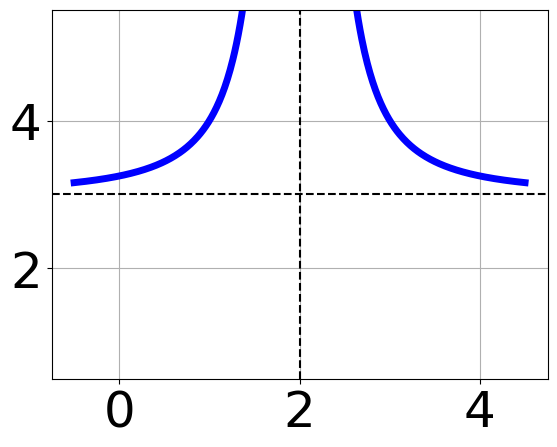
\includegraphics[width=0.3\textwidth]{../Figures/rationalEquationToGraphBB.png}
\end{center}\begin{enumerate}[label=\Alph*.]
\begin{multicols}{2}
\item 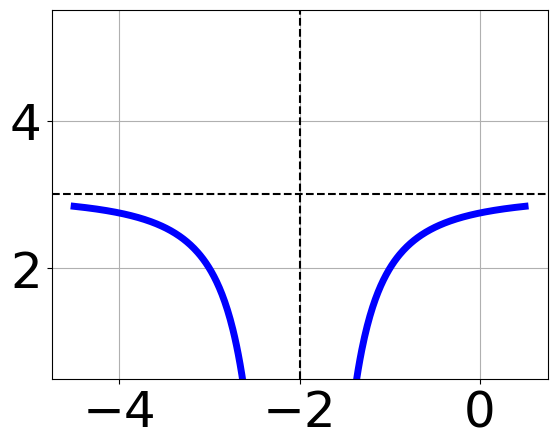
\includegraphics[width = 0.3\textwidth]{../Figures/rationalEquationToGraphAB.png}
\item 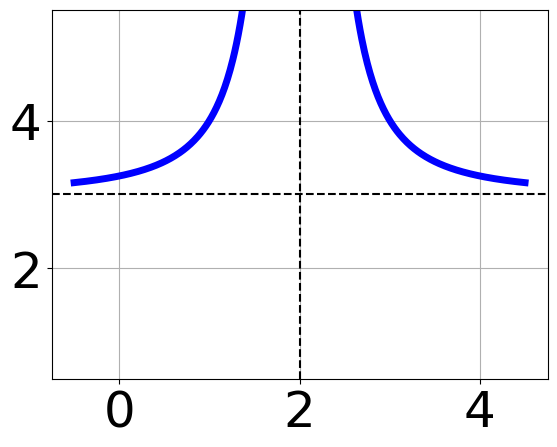
\includegraphics[width = 0.3\textwidth]{../Figures/rationalEquationToGraphBB.png}
\item 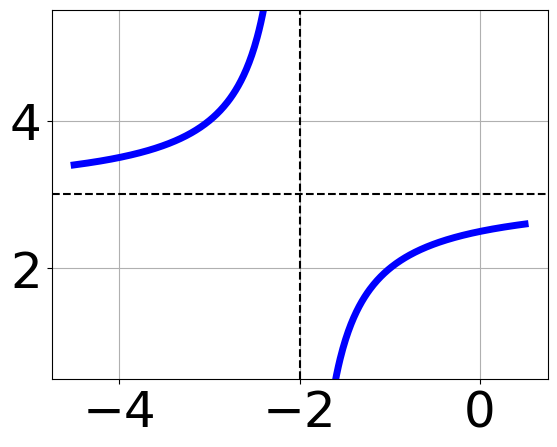
\includegraphics[width = 0.3\textwidth]{../Figures/rationalEquationToGraphCB.png}
\item 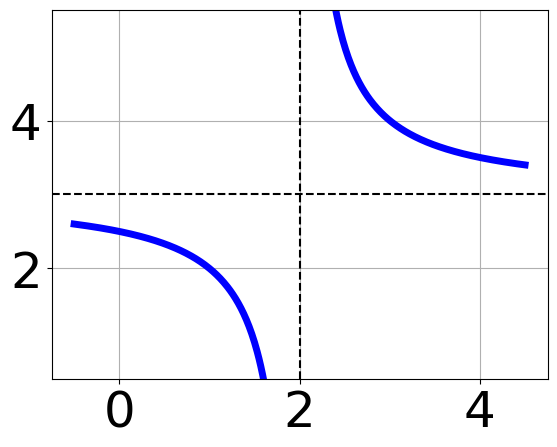
\includegraphics[width = 0.3\textwidth]{../Figures/rationalEquationToGraphDB.png}
\end{multicols}\item None of the above.\end{enumerate}
\textbf{General Comment:} Remember that the general form of a basic rational equation is $ f(x) = \frac{a}{(x-h)^n} + k$, where $a$ is the leading coefficient (and in this case, we assume is either $1$ or $-1$), $n$ is the degree (in this case, either $1$ or $2$), and $(h, k)$ is the intersection of the asymptotes.
}
\litem{
Solve the rational equation below. Then, choose the interval(s) that the solution(s) belongs to.
\[ \frac{-7}{5x -9} + -6 = \frac{-2}{-30x + 54} \]

The solution is \( x = 1.556 \), which is option D.\begin{enumerate}[label=\Alph*.]
\item \( \text{All solutions lead to invalid or complex values in the equation.} \)

This corresponds to thinking $x = 1.556$ leads to dividing by zero in the original equation, which it does not.
\item \( x_1 \in [-3.04, 0.96] \text{ and } x_2 \in [1.47,1.59] \)

$x = -2.044 \text{ and } x = 1.556$, which corresponds to getting the correct solution and believing there should be a second solution to the equation.
\item \( x \in [-3.04,0.96] \)

$x = -2.044$, which corresponds to not distributing the factor $5x -9$ correctly when trying to eliminate the fraction.
\item \( x \in [0.56,3.56] \)

* $x = 1.556$, which is the correct option.
\item \( x_1 \in [0.56, 2.56] \text{ and } x_2 \in [1.57,1.92] \)

$x = 1.556 \text{ and } x = 1.633$, which corresponds to getting the correct solution and believing there should be a second solution to the equation.
\end{enumerate}

\textbf{General Comment:} Distractors are different based on the number of solutions. Remember that after solving, we need to make sure our solution does not make the original equation divide by zero!
}
\litem{
Determine the domain of the function below.
\[ f(x) = \frac{3}{36x^{2} +48 x + 15} \]

The solution is \( \text{All Real numbers except } x = -0.833 \text{ and } x = -0.500. \), which is option D.\begin{enumerate}[label=\Alph*.]
\item \( \text{All Real numbers except } x = a \text{ and } x = b, \text{ where } a \in [-30.12, -29.31] \text{ and } b \in [-18.17, -17.5] \)

All Real numbers except $x = -30.000$ and $x = -18.000$, which corresponds to not factoring the denominator correctly.
\item \( \text{All Real numbers except } x = a, \text{ where } a \in [-30.12, -29.31] \)

All Real numbers except $x = -30.000$, which corresponds to removing a distractor value from the denominator.
\item \( \text{All Real numbers except } x = a, \text{ where } a \in [-0.86, -0.54] \)

All Real numbers except $x = -0.833$, which corresponds to removing only 1 value from the denominator.
\item \( \text{All Real numbers except } x = a \text{ and } x = b, \text{ where } a \in [-0.86, -0.54] \text{ and } b \in [-0.73, 0.03] \)

All Real numbers except $x = -0.833$ and $x = -0.500$, which is the correct option.
\item \( \text{All Real numbers.} \)

This corresponds to thinking the denominator has complex roots or that rational functions have a domain of all Real numbers.
\end{enumerate}

\textbf{General Comment:} Recall that dividing by zero is not a real number. Therefore the domain is all real numbers \textbf{except} those that make the denominator 0.
}
\litem{
Choose the graph of the equation below.
\[ f(x) = \frac{1}{(x - 1)^2} + 2 \]

The solution is the graph below, which is option D.
\begin{center}
    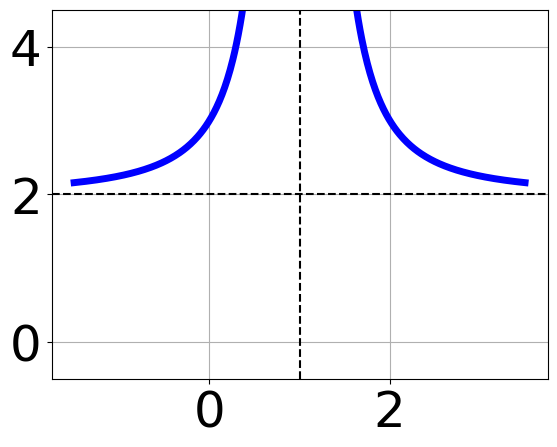
\includegraphics[width=0.3\textwidth]{../Figures/rationalEquationToGraphCopyDB.png}
\end{center}\begin{enumerate}[label=\Alph*.]
\begin{multicols}{2}
\item 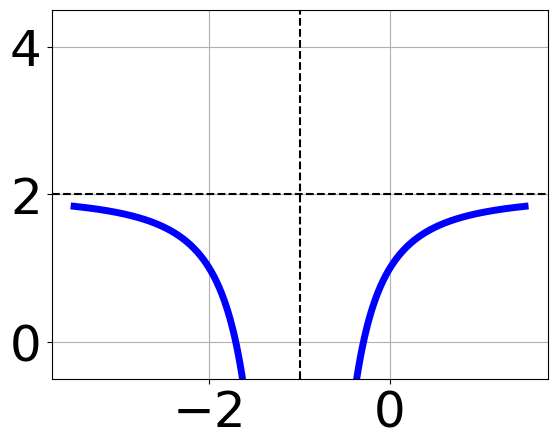
\includegraphics[width = 0.3\textwidth]{../Figures/rationalEquationToGraphCopyAB.png}
\item 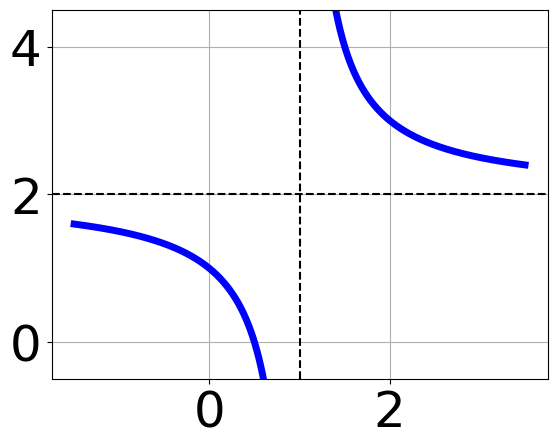
\includegraphics[width = 0.3\textwidth]{../Figures/rationalEquationToGraphCopyBB.png}
\item 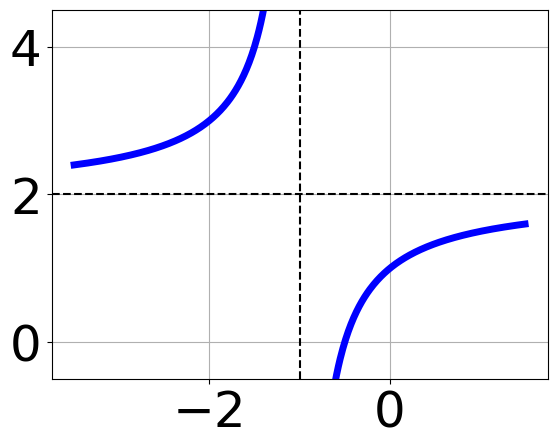
\includegraphics[width = 0.3\textwidth]{../Figures/rationalEquationToGraphCopyCB.png}
\item 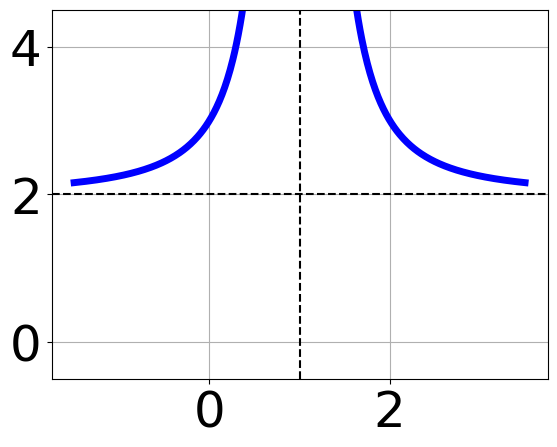
\includegraphics[width = 0.3\textwidth]{../Figures/rationalEquationToGraphCopyDB.png}
\end{multicols}\item None of the above.\end{enumerate}
\textbf{General Comment:} Remember that the general form of a basic rational equation is $ f(x) = \frac{a}{(x-h)^n} + k$, where $a$ is the leading coefficient (and in this case, we assume is either $1$ or $-1$), $n$ is the degree (in this case, either $1$ or $2$), and $(h, k)$ is the intersection of the asymptotes.
}
\litem{
Choose the equation of the function graphed below.

\begin{center}
    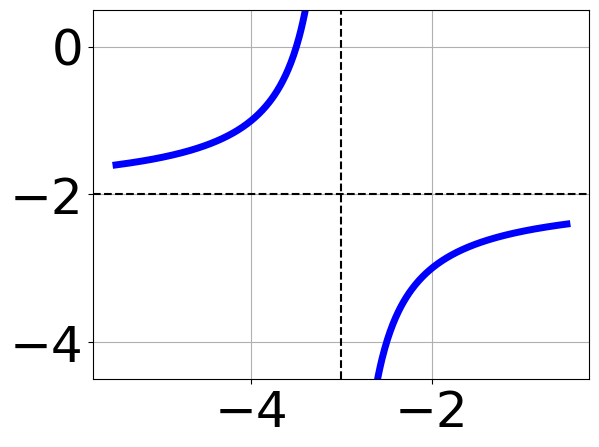
\includegraphics[width=0.5\textwidth]{../Figures/rationalGraphToEquationCopyB.png}
\end{center}




The solution is \( \text{None of the above as it should be } f(x) = \frac{-1}{x + 3} - 2 \), which is option E.\begin{enumerate}[label=\Alph*.]
\item \( f(x) = \frac{1}{(x - 3)^2} - 4 \)

Corresponds to thinking the graph was a shifted version of $\frac{1}{x^2}$, using the general form $f(x) = \frac{a}{x+h}+k$, the opposite leading coefficient, AND not noticing the $y$-value was wrong.
\item \( f(x) = \frac{-1}{x + 3} - 4 \)

The $y$-value of the equation does not match the graph.
\item \( f(x) = \frac{-1}{(x + 3)^2} - 4 \)

Corresponds to thinking the graph was a shifted version of $\frac{1}{x^2}$ not noticing the $y$-value was wrong.
\item \( f(x) = \frac{1}{x - 3} - 4 \)

Corresponds to using the general form $f(x) = \frac{a}{x+h}+k$, the opposite leading coefficient AND not noticing the $y$-value was wrong.
\item \( \text{None of the above} \)

None of the equation options were the correct equation.
\end{enumerate}

\textbf{General Comment:} Remember that the general form of a basic rational equation is $ f(x) = \frac{a}{(x-h)^n} + k$, where $a$ is the leading coefficient (and in this case, we assume is either $1$ or $-1$), $n$ is the degree (in this case, either $1$ or $2$), and $(h, k)$ is the intersection of the asymptotes.
}
\litem{
Solve the rational equation below. Then, choose the interval(s) that the solution(s) belongs to.
\[ \frac{-2x}{2x -7} + \frac{-3x^{2}}{-10x^{2} +25 x + 35} = \frac{-3}{-5x -5} \]

The solution is \( \text{There are two solutions: } x = 0.932 \text{ and } x = -3.218 \), which is option E.\begin{enumerate}[label=\Alph*.]
\item \( x \in [-1.69,0.55] \)


\item \( x_1 \in [0.01, 1.5] \text{ and } x_2 \in [0.5,4.5] \)


\item \( \text{All solutions lead to invalid or complex values in the equation.} \)


\item \( x \in [-3.37,-1.37] \)


\item \( x_1 \in [0.01, 1.5] \text{ and } x_2 \in [-6.22,2.78] \)

* $x = 0.932 \text{ and } x = -3.218$, which is the correct option.
\end{enumerate}

\textbf{General Comment:} Distractors are different based on the number of solutions. Remember that after solving, we need to make sure our solution does not make the original equation divide by zero!
}
\end{enumerate}

\end{document}